\begin{evenBlock}{Four Corner Passing}

\begin{minipage}[t]{\linewidth}
    \centering
    
    \begin{minipage}{.3\linewidth} % Left column and width
        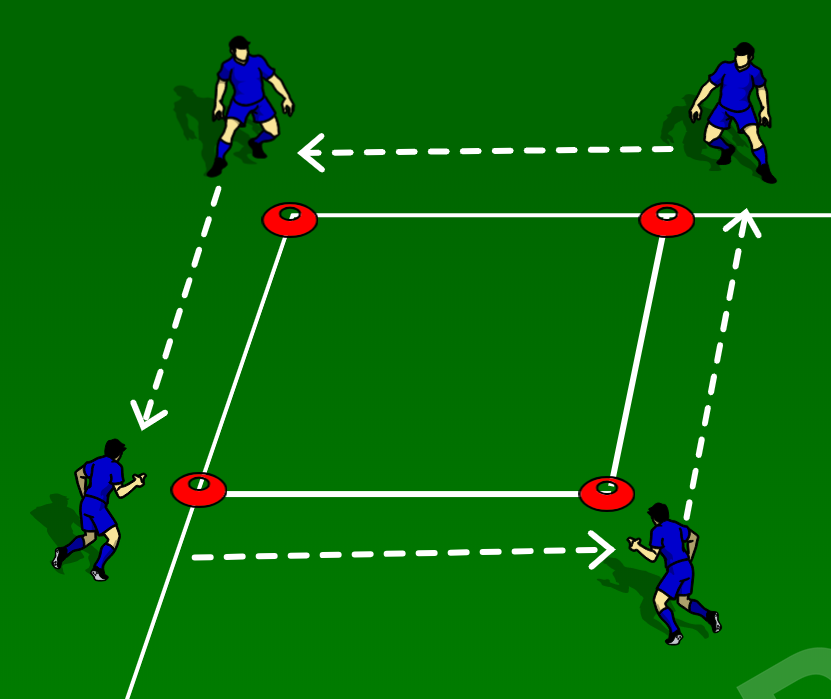
\includegraphics[width=.8\textwidth]{../img/Trimmed/Triangle_Passing_4P_mini}
    \end{minipage}
    \hspace{0.05\linewidth}
    \begin{minipage}{.6\linewidth} % Left column and width
        \textbf{Drill Description:}
        This drill focuses only on passing accurately and using the correct foot for the first touch.  This is like a 3 man passing drill around a box, but with an extra man so there is no movement element which should allow them to focus on the proper technique.
        \begin{enumerate}
            \setlength{\itemsep}{0pt}
            \setlength{\parskip}{0pt}
            \setlength{\parsep}{0pt}
            \item All players stand `open' to they can see all 3 of the players.
            \item The ball should be passed on one direction to start (to the left is more natural for a right footed player).
            \item The player receiving the ball should move his body so he receives the ball on his left foot then passes it to the next player using his right.
            \item After 5 rounds around the box, switch directions.  Pass to the right using the left foot, trap with the right.
        \end{enumerate}
    \end{minipage}

        \raggedright
        \textbf{Coaching Points:}
        \begin{itemize}
            \setlength{\itemsep}{0pt}
            \setlength{\parskip}{0pt}
            \setlength{\parsep}{0pt}
            \item Explain the first touch with the correct foot is the most important part.
            \item The touch should place the ball one step away from the player so they can step into and make a strong pass.
            \item The goal is to use two touches, not 1 and not 3.
            \item Once the passing and trapping with the correct foot becomes more natural, allow then to change directions at will, but any two adjacent players can't pass the ball back and forth more than 3 times.
        \end{itemize}

    
\end{minipage}

\end{evenBlock}